% Options for packages loaded elsewhere
\PassOptionsToPackage{unicode}{hyperref}
\PassOptionsToPackage{hyphens}{url}
\PassOptionsToPackage{dvipsnames,svgnames,x11names}{xcolor}
%
\documentclass[
  letterpaper,
  DIV=11,
  numbers=noendperiod]{scrartcl}

\usepackage{amsmath,amssymb}
\usepackage{iftex}
\ifPDFTeX
  \usepackage[T1]{fontenc}
  \usepackage[utf8]{inputenc}
  \usepackage{textcomp} % provide euro and other symbols
\else % if luatex or xetex
  \usepackage{unicode-math}
  \defaultfontfeatures{Scale=MatchLowercase}
  \defaultfontfeatures[\rmfamily]{Ligatures=TeX,Scale=1}
\fi
\usepackage{lmodern}
\ifPDFTeX\else  
    % xetex/luatex font selection
\fi
% Use upquote if available, for straight quotes in verbatim environments
\IfFileExists{upquote.sty}{\usepackage{upquote}}{}
\IfFileExists{microtype.sty}{% use microtype if available
  \usepackage[]{microtype}
  \UseMicrotypeSet[protrusion]{basicmath} % disable protrusion for tt fonts
}{}
\makeatletter
\@ifundefined{KOMAClassName}{% if non-KOMA class
  \IfFileExists{parskip.sty}{%
    \usepackage{parskip}
  }{% else
    \setlength{\parindent}{0pt}
    \setlength{\parskip}{6pt plus 2pt minus 1pt}}
}{% if KOMA class
  \KOMAoptions{parskip=half}}
\makeatother
\usepackage{xcolor}
\setlength{\emergencystretch}{3em} % prevent overfull lines
\setcounter{secnumdepth}{-\maxdimen} % remove section numbering
% Make \paragraph and \subparagraph free-standing
\makeatletter
\ifx\paragraph\undefined\else
  \let\oldparagraph\paragraph
  \renewcommand{\paragraph}{
    \@ifstar
      \xxxParagraphStar
      \xxxParagraphNoStar
  }
  \newcommand{\xxxParagraphStar}[1]{\oldparagraph*{#1}\mbox{}}
  \newcommand{\xxxParagraphNoStar}[1]{\oldparagraph{#1}\mbox{}}
\fi
\ifx\subparagraph\undefined\else
  \let\oldsubparagraph\subparagraph
  \renewcommand{\subparagraph}{
    \@ifstar
      \xxxSubParagraphStar
      \xxxSubParagraphNoStar
  }
  \newcommand{\xxxSubParagraphStar}[1]{\oldsubparagraph*{#1}\mbox{}}
  \newcommand{\xxxSubParagraphNoStar}[1]{\oldsubparagraph{#1}\mbox{}}
\fi
\makeatother

\usepackage{color}
\usepackage{fancyvrb}
\newcommand{\VerbBar}{|}
\newcommand{\VERB}{\Verb[commandchars=\\\{\}]}
\DefineVerbatimEnvironment{Highlighting}{Verbatim}{commandchars=\\\{\}}
% Add ',fontsize=\small' for more characters per line
\usepackage{framed}
\definecolor{shadecolor}{RGB}{241,243,245}
\newenvironment{Shaded}{\begin{snugshade}}{\end{snugshade}}
\newcommand{\AlertTok}[1]{\textcolor[rgb]{0.68,0.00,0.00}{#1}}
\newcommand{\AnnotationTok}[1]{\textcolor[rgb]{0.37,0.37,0.37}{#1}}
\newcommand{\AttributeTok}[1]{\textcolor[rgb]{0.40,0.45,0.13}{#1}}
\newcommand{\BaseNTok}[1]{\textcolor[rgb]{0.68,0.00,0.00}{#1}}
\newcommand{\BuiltInTok}[1]{\textcolor[rgb]{0.00,0.23,0.31}{#1}}
\newcommand{\CharTok}[1]{\textcolor[rgb]{0.13,0.47,0.30}{#1}}
\newcommand{\CommentTok}[1]{\textcolor[rgb]{0.37,0.37,0.37}{#1}}
\newcommand{\CommentVarTok}[1]{\textcolor[rgb]{0.37,0.37,0.37}{\textit{#1}}}
\newcommand{\ConstantTok}[1]{\textcolor[rgb]{0.56,0.35,0.01}{#1}}
\newcommand{\ControlFlowTok}[1]{\textcolor[rgb]{0.00,0.23,0.31}{\textbf{#1}}}
\newcommand{\DataTypeTok}[1]{\textcolor[rgb]{0.68,0.00,0.00}{#1}}
\newcommand{\DecValTok}[1]{\textcolor[rgb]{0.68,0.00,0.00}{#1}}
\newcommand{\DocumentationTok}[1]{\textcolor[rgb]{0.37,0.37,0.37}{\textit{#1}}}
\newcommand{\ErrorTok}[1]{\textcolor[rgb]{0.68,0.00,0.00}{#1}}
\newcommand{\ExtensionTok}[1]{\textcolor[rgb]{0.00,0.23,0.31}{#1}}
\newcommand{\FloatTok}[1]{\textcolor[rgb]{0.68,0.00,0.00}{#1}}
\newcommand{\FunctionTok}[1]{\textcolor[rgb]{0.28,0.35,0.67}{#1}}
\newcommand{\ImportTok}[1]{\textcolor[rgb]{0.00,0.46,0.62}{#1}}
\newcommand{\InformationTok}[1]{\textcolor[rgb]{0.37,0.37,0.37}{#1}}
\newcommand{\KeywordTok}[1]{\textcolor[rgb]{0.00,0.23,0.31}{\textbf{#1}}}
\newcommand{\NormalTok}[1]{\textcolor[rgb]{0.00,0.23,0.31}{#1}}
\newcommand{\OperatorTok}[1]{\textcolor[rgb]{0.37,0.37,0.37}{#1}}
\newcommand{\OtherTok}[1]{\textcolor[rgb]{0.00,0.23,0.31}{#1}}
\newcommand{\PreprocessorTok}[1]{\textcolor[rgb]{0.68,0.00,0.00}{#1}}
\newcommand{\RegionMarkerTok}[1]{\textcolor[rgb]{0.00,0.23,0.31}{#1}}
\newcommand{\SpecialCharTok}[1]{\textcolor[rgb]{0.37,0.37,0.37}{#1}}
\newcommand{\SpecialStringTok}[1]{\textcolor[rgb]{0.13,0.47,0.30}{#1}}
\newcommand{\StringTok}[1]{\textcolor[rgb]{0.13,0.47,0.30}{#1}}
\newcommand{\VariableTok}[1]{\textcolor[rgb]{0.07,0.07,0.07}{#1}}
\newcommand{\VerbatimStringTok}[1]{\textcolor[rgb]{0.13,0.47,0.30}{#1}}
\newcommand{\WarningTok}[1]{\textcolor[rgb]{0.37,0.37,0.37}{\textit{#1}}}

\providecommand{\tightlist}{%
  \setlength{\itemsep}{0pt}\setlength{\parskip}{0pt}}\usepackage{longtable,booktabs,array}
\usepackage{calc} % for calculating minipage widths
% Correct order of tables after \paragraph or \subparagraph
\usepackage{etoolbox}
\makeatletter
\patchcmd\longtable{\par}{\if@noskipsec\mbox{}\fi\par}{}{}
\makeatother
% Allow footnotes in longtable head/foot
\IfFileExists{footnotehyper.sty}{\usepackage{footnotehyper}}{\usepackage{footnote}}
\makesavenoteenv{longtable}
\usepackage{graphicx}
\makeatletter
\newsavebox\pandoc@box
\newcommand*\pandocbounded[1]{% scales image to fit in text height/width
  \sbox\pandoc@box{#1}%
  \Gscale@div\@tempa{\textheight}{\dimexpr\ht\pandoc@box+\dp\pandoc@box\relax}%
  \Gscale@div\@tempb{\linewidth}{\wd\pandoc@box}%
  \ifdim\@tempb\p@<\@tempa\p@\let\@tempa\@tempb\fi% select the smaller of both
  \ifdim\@tempa\p@<\p@\scalebox{\@tempa}{\usebox\pandoc@box}%
  \else\usebox{\pandoc@box}%
  \fi%
}
% Set default figure placement to htbp
\def\fps@figure{htbp}
\makeatother

\usepackage{booktabs}
\usepackage{longtable}
\usepackage{array}
\usepackage{multirow}
\usepackage{wrapfig}
\usepackage{float}
\usepackage{colortbl}
\usepackage{pdflscape}
\usepackage{tabu}
\usepackage{threeparttable}
\usepackage{threeparttablex}
\usepackage[normalem]{ulem}
\usepackage{makecell}
\usepackage{xcolor}
\KOMAoption{captions}{tableheading}
\makeatletter
\@ifpackageloaded{caption}{}{\usepackage{caption}}
\AtBeginDocument{%
\ifdefined\contentsname
  \renewcommand*\contentsname{Table of contents}
\else
  \newcommand\contentsname{Table of contents}
\fi
\ifdefined\listfigurename
  \renewcommand*\listfigurename{List of Figures}
\else
  \newcommand\listfigurename{List of Figures}
\fi
\ifdefined\listtablename
  \renewcommand*\listtablename{List of Tables}
\else
  \newcommand\listtablename{List of Tables}
\fi
\ifdefined\figurename
  \renewcommand*\figurename{Figure}
\else
  \newcommand\figurename{Figure}
\fi
\ifdefined\tablename
  \renewcommand*\tablename{Table}
\else
  \newcommand\tablename{Table}
\fi
}
\@ifpackageloaded{float}{}{\usepackage{float}}
\floatstyle{ruled}
\@ifundefined{c@chapter}{\newfloat{codelisting}{h}{lop}}{\newfloat{codelisting}{h}{lop}[chapter]}
\floatname{codelisting}{Listing}
\newcommand*\listoflistings{\listof{codelisting}{List of Listings}}
\makeatother
\makeatletter
\makeatother
\makeatletter
\@ifpackageloaded{caption}{}{\usepackage{caption}}
\@ifpackageloaded{subcaption}{}{\usepackage{subcaption}}
\makeatother

\usepackage{bookmark}

\IfFileExists{xurl.sty}{\usepackage{xurl}}{} % add URL line breaks if available
\urlstyle{same} % disable monospaced font for URLs
\hypersetup{
  pdftitle={Final\_Report},
  colorlinks=true,
  linkcolor={blue},
  filecolor={Maroon},
  citecolor={Blue},
  urlcolor={Blue},
  pdfcreator={LaTeX via pandoc}}


\title{Final\_Report}
\author{}
\date{}

\begin{document}
\maketitle


\subsection{1. Project Description}\label{project-description}

Moira Foster was tasked with designing an experiment that measured
helmet foam durability over long periods of time. The experiment
contained three different chemical compositions of foam with two
different porosity levels, to create six types of foam. Each of these
foams were compressed at different frequencies, strains, and stresses
over a period of time. Dr.~Foster has hired \textbf{enter group name
here.} to deterimine which foam type has the most consistent static
stiffness over time with impact. The sample contains 71 different foam
samples across the 6 combinations.

\subsection{1.1 Research Questions}\label{research-questions}

\textbf{Question 1:} Which combination of porosity and chemical index is
best to predict static stiffness over time after accounting for all
other variables?

\subsection{1.2 Variables}\label{variables}

\emph{What is (are) possible explanatory and response variables?
Relevant notes about how each is measured/recorded.}

\emph{A table is recommended here.}

To ensure that we are extracting the information needed, we created two
new variables to be used in our analysis. First, we created a time
variable that was calculated by taking the number of squishes performed
on a foam sample in that current cycle and dividing it by the frequency
of those squishes. Next, we created a relative static stiffness variable
to act as our response variable. This was done by taking every
measurement of static stiffness for a given foam sample and dividing it
by the initial value of static stiffness for that foam sample. This
helps with seeing how the static stiffness changes over time.

Below is a table of the variables we considered in our analysis:

\begin{table}

\caption{\label{tbl-variables}Variables used in Data Analysis}

\centering{

\centering
\begin{tabular}{ll>{\raggedright\arraybackslash}p{8cm}}
\toprule
\multicolumn{3}{c}{ } \\

Name & Type & Notes\\
\midrule
Sample Code & Categorical & Unique identifier for sample of foam\\
Strain & Numerical & Amount of strain tested on foam sample in kPa\\
Relative Porosity & Numerical & The measured porosity of the foam sample after the initial squish\\
Frequency & Numerical & The frequency at which the sample foam was squished\\
Amplitude & Numerical & The amplitude at which the sample foam was squished\\
\addlinespace
Number of Squishes & Numerical & Number of squishes performed on foam at given time\\
Chemical Index & Categorical & Chemical index of given foam sample (Low, Medium, High)\\
Porosity & Categorical & Porosity of given foam sample (Low, High)\\
Relative Static Stiffness & Numerical & Static stiffness of given foam sample relative to the initial value of static stiffness\\
Time & Numerical & Time recorded at each measurement\\
\bottomrule
\end{tabular}

}

\end{table}%

\section{2. Exploratory Data Analysis
(EDA)}\label{exploratory-data-analysis-eda}

To explore what needs to be done for modeling, we perform some
exploratory data analysis.

\begin{figure}

\centering{

\pandocbounded{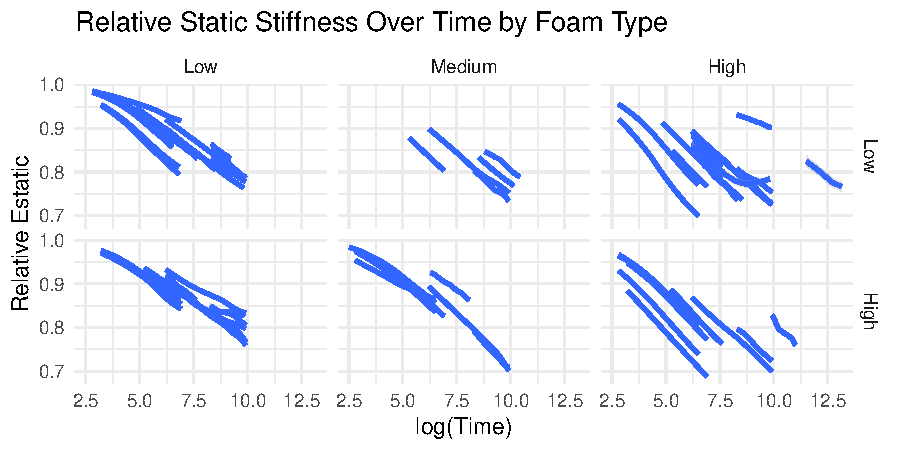
\includegraphics[keepaspectratio]{Final_report_files/figure-pdf/fig-Figure1-1.pdf}}

}

\caption{\label{fig-Figure1}log(Time) vs.~Relative Static Stiffness for
each Foam Type}

\end{figure}%

Figure~\ref{fig-Figure1} shows relative static stiffness over log(Time).
We are using log(Time) because the relationship between time and static
stiffness was not linear. See Figure~\ref{fig-estatRel-time} in the
appendix for more information. From this figure, we can see that there
is a negative relationship between log(Time) and relative static
stiffness. It also appears that, depending on the foam type, there might
be a different relationship. Some slopes are steeper than others, and
some of the starting values of relative static stiffness are different
than others which led us to believe that in the model we would need
unique intercepts and slopes based on the foam type.

Next, we decided to look at the chemical index and porosity of the foams
versus the relative static stiffness.

\begin{figure}

\centering{

\pandocbounded{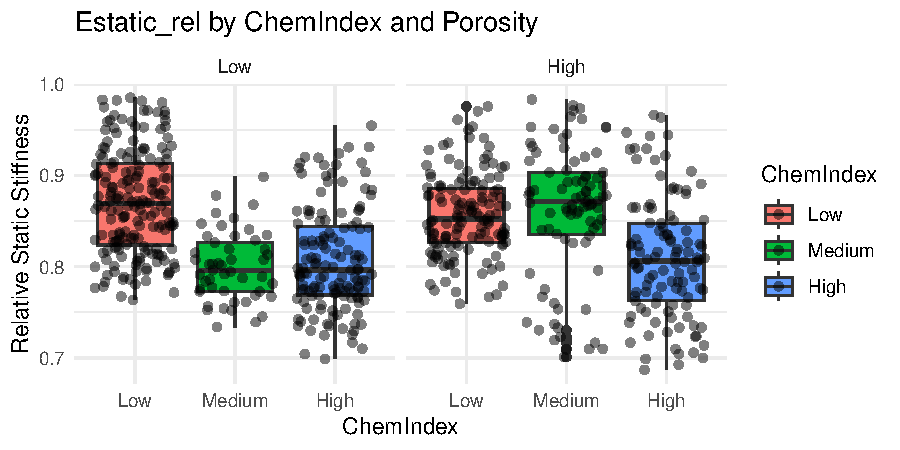
\includegraphics[keepaspectratio]{Final_report_files/figure-pdf/fig-chem-poro-1.pdf}}

}

\caption{\label{fig-chem-poro}Chemical Index vs.~Relative Static
Stiffness for each level of Porosity}

\end{figure}%

In Figure~\ref{fig-chem-poro}, the relationship between chemical index
and relative static stiffness is different for the two levels of foam
porosity. This indicates that there is likely a significant interaction
between chemical index and porosity.

Next, we look at a correlation plot between all numerical variables.

\begin{figure}

\centering{

\pandocbounded{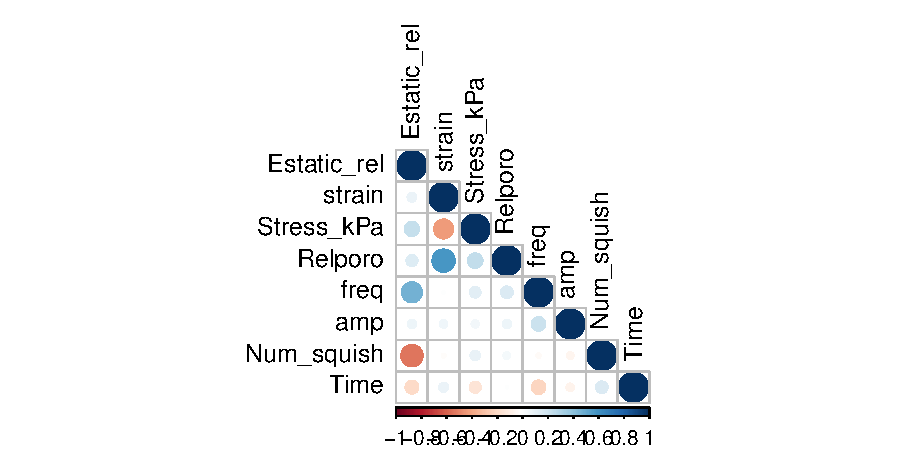
\includegraphics[keepaspectratio]{Final_report_files/figure-pdf/fig-correlation-1.pdf}}

}

\caption{\label{fig-correlation}Correlation Matrix}

\end{figure}%

Figure~\ref{fig-correlation} gives us a good idea of what variables
might need to be included in our final model. As we can see, number of
squishes and frequency are highly correlated with relative static
stiffness. This is obvious, as relative static stiffness is going to
have a relationship with time as we saw in Figure~\ref{fig-Figure1}. We
also see that relative porosity and strain are correlated, as well as
stress and strain.

Lastly, we look at how frequency is related to relative static stiffness
over time.

\begin{figure}

\centering{

\pandocbounded{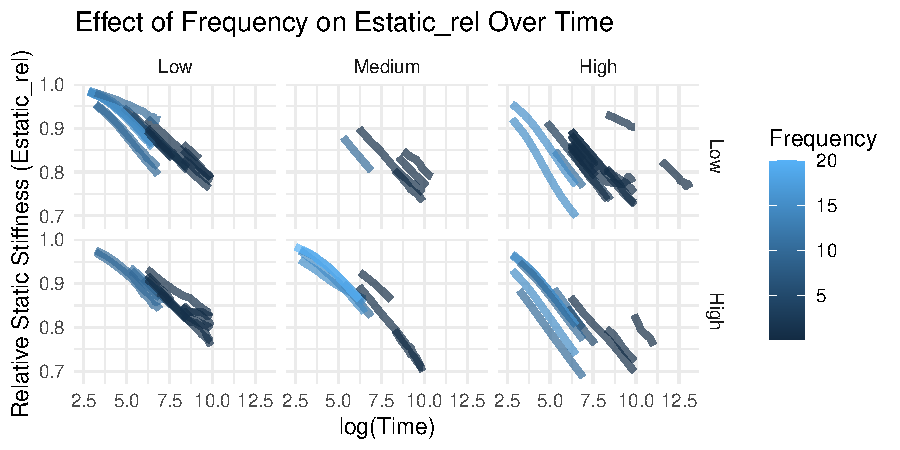
\includegraphics[keepaspectratio]{Final_report_files/figure-pdf/fig-freq-estaticRel-1.pdf}}

}

\caption{\label{fig-freq-estaticRel}Frequency vs.~Relative Static
Stiffness over Time}

\end{figure}%

\textless\textless\textless\textless\textless\textless\textless{} HEAD

In Figure~\ref{fig-freq-estaticRel}, we can see that for lower
frequencies, there is a higher relative static stiffness level recorded.
This trend is the same across the different foam types. Frequency is a
possible explanatory variable that we will consider in our final model.

\section{3. Statistical Analysis}\label{statistical-analysis}

The linear mixed effects model is defined as:

\[
\begin{align*}
Estatic\_rel_{ij} &= \underbrace{\beta_0}_{\text{fixed intercept}} + \underbrace{a_j}_{\text{random intercept for SampleCode}} \\
&\quad + \beta_1 \left(\log(\text{Time}) \cdot \text{Porosity} \right)_{ij} \\
&\quad + \beta_2 \left(\log(\text{Time}) \cdot \text{Porosity} \cdot \text{ChemIndex} \right)_{ij} \\
&\quad + \beta_3 \cdot \text{freq}_{ij} + \beta_4 \cdot \text{numSquish}_{ij} + \varepsilon_{ij}
\end{align*}
\] where:

\(\beta_0\) is the fixed intercept
\(a_j \sim \mathcal{N}(0, \sigma^2_{SampleCode})\) is the random
intercept for group \(j\) (\texttt{SampleCode})
\(\varepsilon_{ij} \sim \mathcal{N}(0, \sigma^2)\) is the residual
error.

\begin{verbatim}
                             numDF denDF   F-value p-value
(Intercept)                      1   622 25384.644  <.0001
ChemIndex                        2    67     9.143   3e-04
freq                             1    67    24.626  <.0001
Num_squish                       1   622 10313.149  <.0001
log(Time):Porosity               2   622  1143.459  <.0001
log(Time):Porosity:ChemIndex     4   622    63.594  <.0001
\end{verbatim}

In the table above, we can see that all terms included in the model are
significant with p-values \(< .0001\).

The figure below shows the the emmean of our model, sorted by foam type.

\begin{figure}[H]

{\centering \pandocbounded{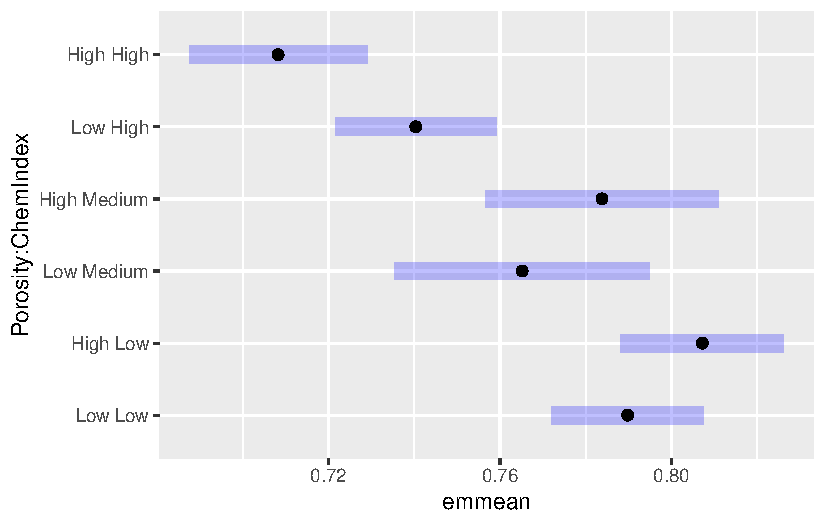
\includegraphics[keepaspectratio]{Final_report_files/figure-pdf/em-plot-1.pdf}}

}

\caption{Emmeans Comparison by Porosity*ChemIndex}

\end{figure}%

\section{4. Recommendations}\label{recommendations}

\textbf{Question 1:} Which combination of porosity and chemical index is
best at keeping static stiffness stable over time, after accounting for
all other variables?

For the most consistent static stiffness, a foam with high porosity and
a low chemical index will be best.

\section{5. Resources}\label{resources}

\emph{List resources that your client might find useful}

\section{6. Additional Considerations}\label{additional-considerations}

\begin{itemize}
\tightlist
\item
  \emph{Limitations to the recommendations}
\item
  \emph{Concerns you may have about the study; suggestions for similar
  studies in future}
\item
  \emph{Technical comments}
\end{itemize}

\section{Technical Appendix}\label{technical-appendix}

\begin{figure}

\centering{

\pandocbounded{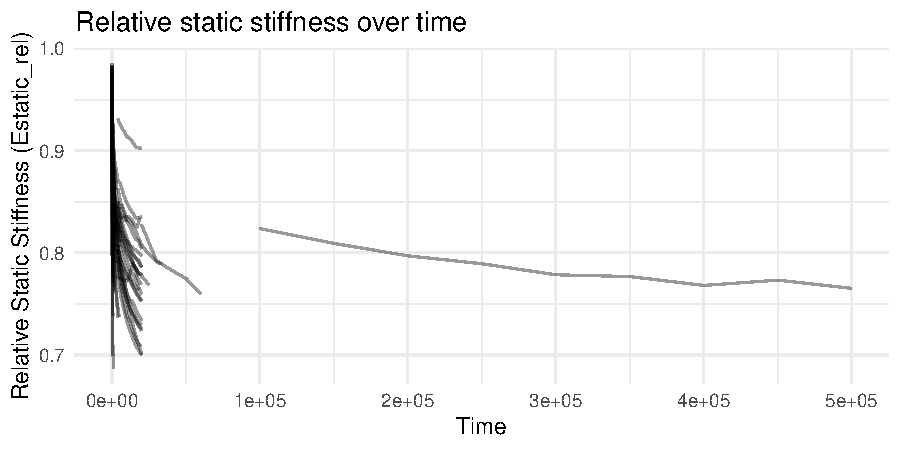
\includegraphics[keepaspectratio]{Final_report_files/figure-pdf/fig-estatRel-time-1.pdf}}

}

\caption{\label{fig-estatRel-time}Time vs.~Relative Static Stiffness}

\end{figure}%

Here we can see a clear nonlinear relationship between relative static
stiffness and time. A logarithmic transformation is needed. See
Figure~\ref{fig-estatRel-logTime}.

\begin{figure}

\centering{

\pandocbounded{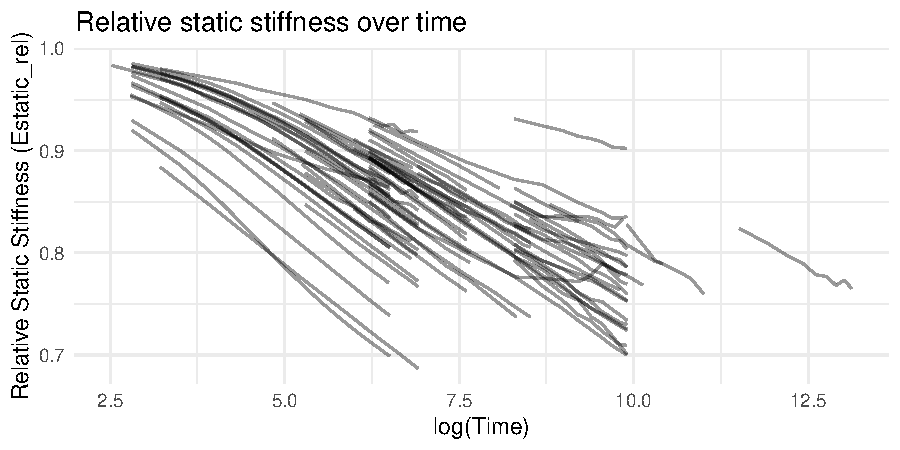
\includegraphics[keepaspectratio]{Final_report_files/figure-pdf/fig-estatRel-logTime-1.pdf}}

}

\caption{\label{fig-estatRel-logTime}log(Time) vs.~Relative Static
Stiffness}

\end{figure}%

\pandocbounded{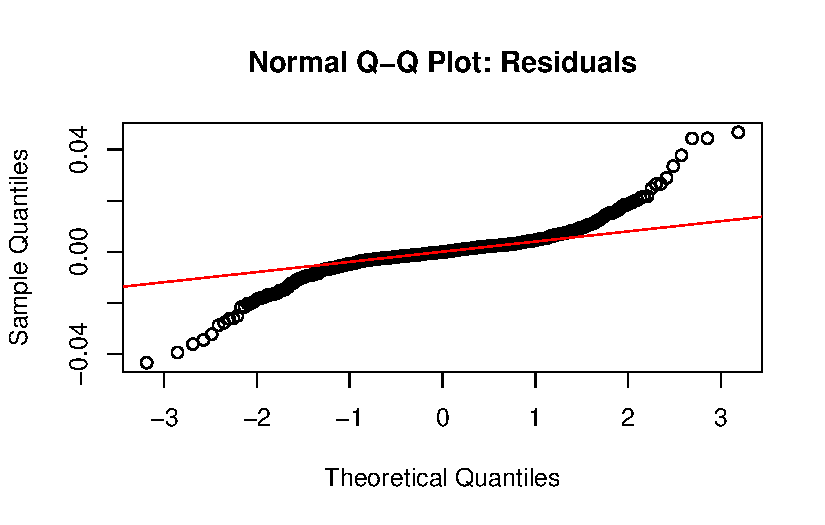
\includegraphics[keepaspectratio]{Final_report_files/figure-pdf/diag-plots-1.pdf}}

\pandocbounded{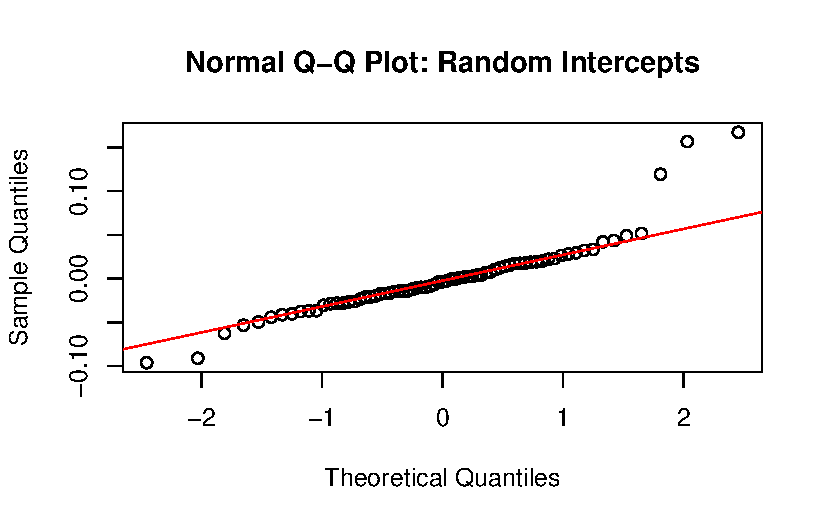
\includegraphics[keepaspectratio]{Final_report_files/figure-pdf/diag-plots-2.pdf}}

\pandocbounded{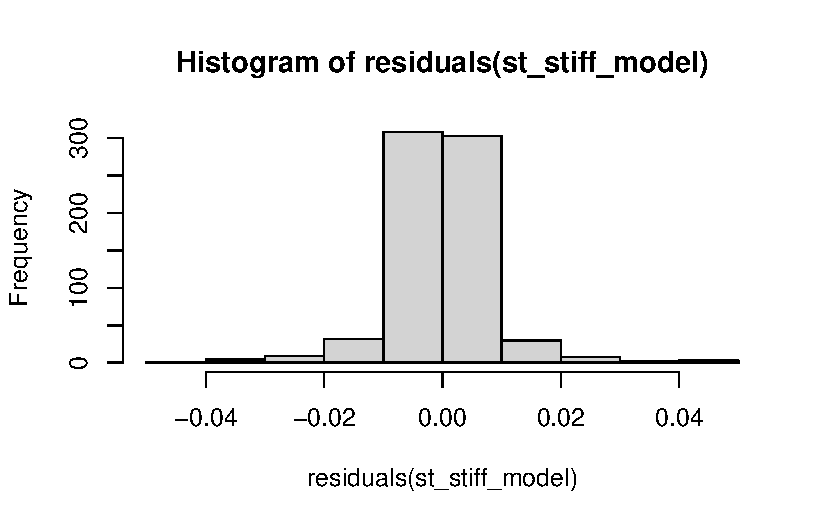
\includegraphics[keepaspectratio]{Final_report_files/figure-pdf/diag-plots-3.pdf}}

\pandocbounded{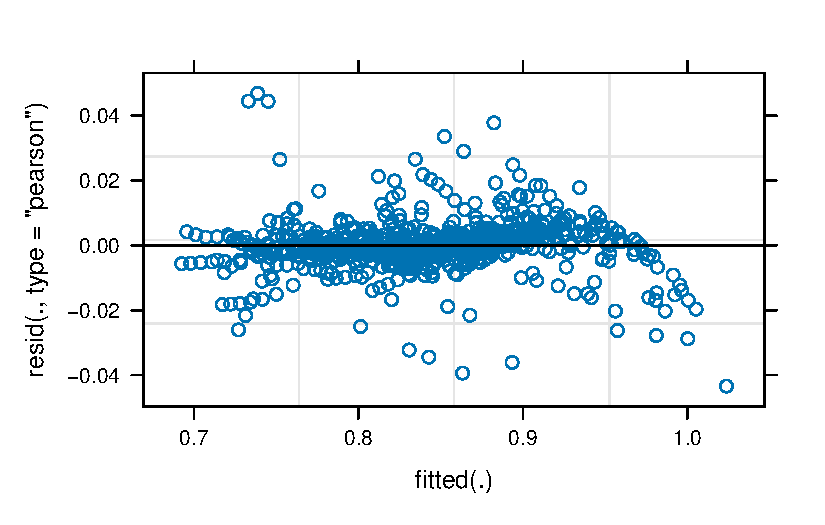
\includegraphics[keepaspectratio]{Final_report_files/figure-pdf/diag-plots-4.pdf}}

\subsubsection{R Script}\label{r-script}

\begin{Shaded}
\begin{Highlighting}[]
\CommentTok{\# clean up \& set default chunk options}
\FunctionTok{rm}\NormalTok{(}\AttributeTok{list =} \FunctionTok{ls}\NormalTok{())}
\NormalTok{knitr}\SpecialCharTok{::}\NormalTok{opts\_chunk}\SpecialCharTok{$}\FunctionTok{set}\NormalTok{(}\AttributeTok{echo =} \ConstantTok{FALSE}\NormalTok{)}

\CommentTok{\# packages}
\FunctionTok{library}\NormalTok{(tidyverse) }\CommentTok{\# for example}
\FunctionTok{library}\NormalTok{(mosaic)    }\CommentTok{\# for example}
\FunctionTok{library}\NormalTok{(ggformula) }\CommentTok{\# for example}
\FunctionTok{library}\NormalTok{(lme4)}
\FunctionTok{library}\NormalTok{(ggplot2)}
\FunctionTok{library}\NormalTok{(emmeans)}
\FunctionTok{library}\NormalTok{(nlme)}
\FunctionTok{library}\NormalTok{(readxl)}
\FunctionTok{library}\NormalTok{(tinytex) }
\FunctionTok{library}\NormalTok{(xtable)}
\FunctionTok{library}\NormalTok{(knitr)}
\FunctionTok{library}\NormalTok{(ggthemes)}
\FunctionTok{library}\NormalTok{(GGally)}
\FunctionTok{library}\NormalTok{(kableExtra)}
\FunctionTok{library}\NormalTok{(emmeans)}
\FunctionTok{library}\NormalTok{(Stat2Data)}
\FunctionTok{library}\NormalTok{(corrplot)}


\CommentTok{\# read in data }

\CommentTok{\# use this space to do any data processing you need}

\CommentTok{\# load data}
\NormalTok{df }\OtherTok{\textless{}{-}} \FunctionTok{read\_xlsx}\NormalTok{(}\StringTok{"Foster\_Mines\_Capstone\_Data\_v2.xlsx"}\NormalTok{)}

\CommentTok{\#Pivot all cycle{-}related columns into long format}
\NormalTok{df\_long }\OtherTok{\textless{}{-}}\NormalTok{ df }\SpecialCharTok{\%\textgreater{}\%}
  \FunctionTok{pivot\_longer}\NormalTok{(}
    \AttributeTok{cols =} \FunctionTok{matches}\NormalTok{(}\StringTok{"(\^{}Cyc\_[A{-}Z]$)|(\_Cyc\_[A{-}Z]$)"}\NormalTok{),}
    \AttributeTok{names\_to =} \StringTok{"FullName"}\NormalTok{,       }\CommentTok{\# give it a neutral name}
    \AttributeTok{values\_to =} \StringTok{"Value"}
\NormalTok{  )}

\CommentTok{\#Extract the cycle (e.g., Cyc\_A) and variable type (e.g., E1\_MPA)}
\NormalTok{df\_tidy }\OtherTok{\textless{}{-}}\NormalTok{ df\_long }\SpecialCharTok{\%\textgreater{}\%}
  \FunctionTok{mutate}\NormalTok{(}
    \AttributeTok{Cycle =} \FunctionTok{str\_extract}\NormalTok{(FullName, }\StringTok{"Cyc\_[A{-}Z]$"}\NormalTok{),}
    \AttributeTok{VariableType =} \FunctionTok{str\_remove}\NormalTok{(FullName, }\StringTok{"\_Cyc\_[A{-}Z]$"}\NormalTok{),}
    \AttributeTok{VariableType =} \FunctionTok{ifelse}\NormalTok{(VariableType }\SpecialCharTok{==} \StringTok{"Cyc"}\NormalTok{, }\StringTok{"Cycle\_time"}\NormalTok{, VariableType)}
\NormalTok{  ) }\SpecialCharTok{\%\textgreater{}\%}
  \FunctionTok{select}\NormalTok{(}\SpecialCharTok{{-}}\NormalTok{FullName) }\SpecialCharTok{\%\textgreater{}\%}
  \FunctionTok{pivot\_wider}\NormalTok{(}
    \AttributeTok{names\_from =}\NormalTok{ VariableType,}
    \AttributeTok{values\_from =}\NormalTok{ Value}
\NormalTok{  ) }\SpecialCharTok{\%\textgreater{}\%}
  \FunctionTok{arrange}\NormalTok{(SampleCode, Cycle)}

\FunctionTok{head}\NormalTok{(df\_tidy)}

\CommentTok{\#Pivot the actual cycle time columns only}
\NormalTok{df\_lt }\OtherTok{\textless{}{-}}\NormalTok{ df\_tidy }\SpecialCharTok{\%\textgreater{}\%}
  \FunctionTok{pivot\_longer}\NormalTok{(}
    \AttributeTok{cols =} \FunctionTok{matches}\NormalTok{(}\StringTok{"\^{}Cyc\_[A{-}Z]$"}\NormalTok{),  }\CommentTok{\# Cyc\_A to Cyc\_N}
    \AttributeTok{names\_to =} \StringTok{"Cycle\_column"}\NormalTok{,      }\CommentTok{\# Temporary name to avoid collision}
    \AttributeTok{values\_to =} \StringTok{"Num\_squish"}
\NormalTok{  )}

\CommentTok{\#Remove NA times}
\NormalTok{df\_clean }\OtherTok{\textless{}{-}}\NormalTok{ df\_lt }\SpecialCharTok{\%\textgreater{}\%}
  \FunctionTok{filter}\NormalTok{(}\SpecialCharTok{!}\FunctionTok{is.na}\NormalTok{(Num\_squish)) }\SpecialCharTok{\%\textgreater{}\%}
  \FunctionTok{select}\NormalTok{(}\SpecialCharTok{{-}}\NormalTok{Cycle) }\SpecialCharTok{\%\textgreater{}\%}                \CommentTok{\#Drop the existing "Cycle" column and rename}
  \FunctionTok{rename}\NormalTok{(}\AttributeTok{Cycle =}\NormalTok{ Cycle\_column)  }

\NormalTok{df\_clean }\OtherTok{\textless{}{-}}\NormalTok{ df\_clean }\SpecialCharTok{|\textgreater{}}
  \FunctionTok{mutate}\NormalTok{(}
    \AttributeTok{ChemIndex =} \FunctionTok{as.numeric}\NormalTok{(}\FunctionTok{str\_split\_fixed}\NormalTok{(SampleCode, }\StringTok{"\_"}\NormalTok{, }\DecValTok{4}\NormalTok{)[,}\DecValTok{2}\NormalTok{]),}
    \AttributeTok{Porosity =} \FunctionTok{as.numeric}\NormalTok{(}\FunctionTok{str\_split\_fixed}\NormalTok{(SampleCode, }\StringTok{"\_"}\NormalTok{, }\DecValTok{4}\NormalTok{)[,}\DecValTok{3}\NormalTok{]))}

\NormalTok{df\_clean }\OtherTok{\textless{}{-}}\NormalTok{ df\_clean }\SpecialCharTok{\%\textgreater{}\%}
  \FunctionTok{group\_by}\NormalTok{(SampleCode) }\SpecialCharTok{\%\textgreater{}\%}
  \FunctionTok{mutate}\NormalTok{(}
    \AttributeTok{Estatic\_initial =} \FunctionTok{first}\NormalTok{(Estatic\_MPA),  }\CommentTok{\# First Estatic value per SampleCode}
    \AttributeTok{Estatic\_rel =}\NormalTok{ Estatic\_MPA }\SpecialCharTok{/}\NormalTok{ Estatic\_initial  }\CommentTok{\# Relative to initial}
\NormalTok{  ) }\SpecialCharTok{\%\textgreater{}\%}
  \FunctionTok{ungroup}\NormalTok{()}

\NormalTok{df\_clean }\OtherTok{\textless{}{-}}\NormalTok{ df\_clean }\SpecialCharTok{|\textgreater{}}
  \FunctionTok{select}\NormalTok{(}\SpecialCharTok{{-}}\NormalTok{E1\_MPA, }\SpecialCharTok{{-}}\NormalTok{tandelta, }\SpecialCharTok{{-}}\NormalTok{NVP)}

\NormalTok{df\_clean }\OtherTok{\textless{}{-}}\NormalTok{ df\_clean }\SpecialCharTok{\%\textgreater{}\%}
   \FunctionTok{mutate}\NormalTok{(}\AttributeTok{Porosity =} \FunctionTok{case\_when}\NormalTok{(}
\NormalTok{     Porosity }\SpecialCharTok{==} \DecValTok{71} \SpecialCharTok{\textasciitilde{}} \StringTok{"Low"}\NormalTok{,}
\NormalTok{     Porosity }\SpecialCharTok{==} \DecValTok{81} \SpecialCharTok{\textasciitilde{}} \StringTok{"High"}
\NormalTok{   ))}
 
\NormalTok{ df\_clean }\OtherTok{\textless{}{-}}\NormalTok{ df\_clean }\SpecialCharTok{\%\textgreater{}\%}
   \FunctionTok{mutate}\NormalTok{(}\AttributeTok{ChemIndex =} \FunctionTok{case\_when}\NormalTok{(}
\NormalTok{     ChemIndex }\SpecialCharTok{==} \DecValTok{121} \SpecialCharTok{\textasciitilde{}} \StringTok{"High"}\NormalTok{,}
\NormalTok{     ChemIndex }\SpecialCharTok{==} \DecValTok{100} \SpecialCharTok{\textasciitilde{}} \StringTok{"Medium"}\NormalTok{,}
\NormalTok{     ChemIndex }\SpecialCharTok{==} \DecValTok{79} \SpecialCharTok{\textasciitilde{}} \StringTok{"Low"}
\NormalTok{   ))}
 
\NormalTok{ df\_clean}\SpecialCharTok{$}\NormalTok{Porosity }\OtherTok{\textless{}{-}} \FunctionTok{factor}\NormalTok{(df\_clean}\SpecialCharTok{$}\NormalTok{Porosity, }\AttributeTok{levels =} \FunctionTok{c}\NormalTok{(}\StringTok{"Low"}\NormalTok{, }\StringTok{"High"}\NormalTok{))}
 
\NormalTok{ df\_clean}\SpecialCharTok{$}\NormalTok{ChemIndex }\OtherTok{\textless{}{-}} \FunctionTok{factor}\NormalTok{(df\_clean}\SpecialCharTok{$}\NormalTok{ChemIndex, }\AttributeTok{levels =} \FunctionTok{c}\NormalTok{(}\StringTok{"Low"}\NormalTok{, }\StringTok{"Medium"}\NormalTok{, }\StringTok{"High"}\NormalTok{))}
 
\NormalTok{ df\_clean }\OtherTok{\textless{}{-}}\NormalTok{ df\_clean }\SpecialCharTok{\%\textgreater{}\%}
   \FunctionTok{mutate}\NormalTok{(}\AttributeTok{Cycle =} \FunctionTok{case\_when}\NormalTok{(}
\NormalTok{     Cycle }\SpecialCharTok{==} \StringTok{"Cyc\_A"} \SpecialCharTok{\textasciitilde{}} \StringTok{"A"}\NormalTok{,}
\NormalTok{     Cycle }\SpecialCharTok{==} \StringTok{"Cyc\_B"} \SpecialCharTok{\textasciitilde{}} \StringTok{"B"}\NormalTok{,}
\NormalTok{     Cycle }\SpecialCharTok{==} \StringTok{"Cyc\_C"} \SpecialCharTok{\textasciitilde{}} \StringTok{"C"}\NormalTok{,}
\NormalTok{     Cycle }\SpecialCharTok{==} \StringTok{"Cyc\_D"} \SpecialCharTok{\textasciitilde{}} \StringTok{"D"}\NormalTok{,}
\NormalTok{     Cycle }\SpecialCharTok{==} \StringTok{"Cyc\_E"} \SpecialCharTok{\textasciitilde{}} \StringTok{"E"}\NormalTok{,}
\NormalTok{     Cycle }\SpecialCharTok{==} \StringTok{"Cyc\_F"} \SpecialCharTok{\textasciitilde{}} \StringTok{"F"}\NormalTok{,}
\NormalTok{     Cycle }\SpecialCharTok{==} \StringTok{"Cyc\_G"} \SpecialCharTok{\textasciitilde{}} \StringTok{"G"}\NormalTok{,}
\NormalTok{     Cycle }\SpecialCharTok{==} \StringTok{"Cyc\_H"} \SpecialCharTok{\textasciitilde{}} \StringTok{"H"}\NormalTok{,}
\NormalTok{     Cycle }\SpecialCharTok{==} \StringTok{"Cyc\_I"} \SpecialCharTok{\textasciitilde{}} \StringTok{"I"}\NormalTok{,}
\NormalTok{     Cycle }\SpecialCharTok{==} \StringTok{"Cyc\_J"} \SpecialCharTok{\textasciitilde{}} \StringTok{"J"}\NormalTok{,}
\NormalTok{     Cycle }\SpecialCharTok{==} \StringTok{"Cyc\_K"} \SpecialCharTok{\textasciitilde{}} \StringTok{"K"}\NormalTok{,}
\NormalTok{     Cycle }\SpecialCharTok{==} \StringTok{"Cyc\_L"} \SpecialCharTok{\textasciitilde{}} \StringTok{"L"}\NormalTok{,}
\NormalTok{     Cycle }\SpecialCharTok{==} \StringTok{"Cyc\_M"} \SpecialCharTok{\textasciitilde{}} \StringTok{"M"}\NormalTok{,}
\NormalTok{     Cycle }\SpecialCharTok{==} \StringTok{"Cyc\_N"} \SpecialCharTok{\textasciitilde{}} \StringTok{"N"}
\NormalTok{   ))}
 
\NormalTok{ df\_clean}\SpecialCharTok{$}\NormalTok{Cycle }\OtherTok{\textless{}{-}} \FunctionTok{factor}\NormalTok{(df\_clean}\SpecialCharTok{$}\NormalTok{Cycle,}
                          \AttributeTok{levels =} \FunctionTok{c}\NormalTok{(}\StringTok{"A"}\NormalTok{, }\StringTok{"B"}\NormalTok{, }\StringTok{"C"}\NormalTok{, }\StringTok{"D"}\NormalTok{, }\StringTok{"E"}\NormalTok{, }\StringTok{"F"}\NormalTok{, }\StringTok{"G"}\NormalTok{, }\StringTok{"H"}\NormalTok{, }\StringTok{"I"}\NormalTok{, }\StringTok{"J"}\NormalTok{, }\StringTok{"K"}\NormalTok{, }\StringTok{"L"}\NormalTok{, }\StringTok{"M"}\NormalTok{, }\StringTok{"N"}\NormalTok{))}
 
\NormalTok{ df\_clean }\OtherTok{\textless{}{-}}\NormalTok{ df\_clean }\SpecialCharTok{\%\textgreater{}\%}
   \FunctionTok{filter}\NormalTok{(Num\_squish }\SpecialCharTok{\textless{}=} \DecValTok{10000}\NormalTok{)}
\NormalTok{ df\_clean }\OtherTok{\textless{}{-}}\NormalTok{ df\_clean }\SpecialCharTok{\%\textgreater{}\%}
   \FunctionTok{mutate}\NormalTok{(}\AttributeTok{Time =}\NormalTok{ Num\_squish}\SpecialCharTok{/}\NormalTok{freq)}
 
\NormalTok{ df\_clean }\OtherTok{\textless{}{-}}\NormalTok{ df\_clean }\SpecialCharTok{|\textgreater{}}
   \FunctionTok{filter}\NormalTok{(Estatic\_rel }\SpecialCharTok{\textless{}} \DecValTok{1}\NormalTok{)}
 
\NormalTok{variable.desc }\OtherTok{\textless{}{-}} \FunctionTok{data.frame}\NormalTok{(}\AttributeTok{Name =} \FunctionTok{c}\NormalTok{(}\StringTok{"Sample Code"}\NormalTok{, }\StringTok{"Strain"}\NormalTok{, }\StringTok{"Relative Porosity"}\NormalTok{, }\StringTok{"Frequency"}\NormalTok{, }\StringTok{"Amplitude"}\NormalTok{, }\StringTok{"Number of Squishes"}\NormalTok{, }\StringTok{"Chemical Index"}\NormalTok{, }\StringTok{"Porosity"}\NormalTok{, }\StringTok{"Relative Static Stiffness"}\NormalTok{, }\StringTok{"Time"}\NormalTok{))}
\NormalTok{variable.desc}\SpecialCharTok{$}\NormalTok{Type }\OtherTok{\textless{}{-}} \FunctionTok{c}\NormalTok{(}\StringTok{"Categorical"}\NormalTok{, }\StringTok{"Numerical"}\NormalTok{, }\StringTok{"Numerical"}\NormalTok{, }\StringTok{"Numerical"}\NormalTok{, }\StringTok{"Numerical"}\NormalTok{, }\StringTok{"Numerical"}\NormalTok{, }\StringTok{"Categorical"}\NormalTok{, }\StringTok{"Categorical"}\NormalTok{, }\StringTok{"Numerical"}\NormalTok{, }\StringTok{"Numerical"}\NormalTok{)}
\NormalTok{variable.desc}\SpecialCharTok{$}\NormalTok{Notes }\OtherTok{\textless{}{-}} \FunctionTok{c}\NormalTok{(}\StringTok{"Unique identifier for sample of foam"}\NormalTok{, }\StringTok{"Amount of strain tested on foam sample in kPa"}\NormalTok{, }\StringTok{"The measured porosity of the foam sample after the initial squish"}\NormalTok{, }\StringTok{"The frequency at which the sample foam was squished"}\NormalTok{, }\StringTok{"The amplitude at which the sample foam was squished"}\NormalTok{, }\StringTok{"Number of squishes performed on foam at given time"}\NormalTok{, }\StringTok{"Chemical index of given foam sample (Low, Medium, High)"}\NormalTok{, }\StringTok{"Porosity of given foam sample (Low, High)"}\NormalTok{, }\StringTok{"Static stiffness of given foam sample relative to the initial value of static stiffness"}\NormalTok{, }\StringTok{"Time recorded at each measurement"}\NormalTok{)}
\NormalTok{knitr}\SpecialCharTok{::}\FunctionTok{kable}\NormalTok{(variable.desc, }\AttributeTok{format =} \StringTok{"latex"}\NormalTok{, }\AttributeTok{booktabs =} \ConstantTok{TRUE}\NormalTok{,}
             \AttributeTok{col.names =} \FunctionTok{c}\NormalTok{(}\StringTok{"Name"}\NormalTok{, }\StringTok{"Type"}\NormalTok{, }\StringTok{"Notes"}\NormalTok{),}
             \AttributeTok{longtable =} \ConstantTok{FALSE}\NormalTok{) }\SpecialCharTok{\%\textgreater{}\%}
  \FunctionTok{kable\_styling}\NormalTok{( }\AttributeTok{full\_width =} \ConstantTok{FALSE}\NormalTok{) }\SpecialCharTok{\%\textgreater{}\%}
  \FunctionTok{column\_spec}\NormalTok{(}\DecValTok{3}\NormalTok{, }\AttributeTok{width =} \StringTok{"8cm"}\NormalTok{) }\SpecialCharTok{\%\textgreater{}\%} 
  \FunctionTok{add\_header\_above}\NormalTok{(}\FunctionTok{c}\NormalTok{(}\StringTok{" "} \OtherTok{=} \DecValTok{3}\NormalTok{))}
\FunctionTok{ggplot}\NormalTok{(df\_clean, }\FunctionTok{aes}\NormalTok{(}\AttributeTok{x =} \FunctionTok{log}\NormalTok{(Time), }\AttributeTok{y =}\NormalTok{ Estatic\_rel, }\AttributeTok{group =}\NormalTok{ SampleCode)) }\SpecialCharTok{+}
  \FunctionTok{geom\_smooth}\NormalTok{(}\AttributeTok{alpha =} \FloatTok{0.3}\NormalTok{) }\SpecialCharTok{+}
 \CommentTok{\# stat\_summary(aes(group = 1), fun = mean, geom = "line", color = "black", size = 1) +}
  \FunctionTok{facet\_grid}\NormalTok{(Porosity }\SpecialCharTok{\textasciitilde{}}\NormalTok{ ChemIndex) }\SpecialCharTok{+}
  \FunctionTok{labs}\NormalTok{(}\AttributeTok{title =} \StringTok{"Relative Static Stiffness Over Time by Foam Type"}\NormalTok{,}
       \AttributeTok{x =} \StringTok{"log(Time)"}\NormalTok{,}
       \AttributeTok{y =} \StringTok{"Relative Estatic"}\NormalTok{) }\SpecialCharTok{+}
  \FunctionTok{theme\_minimal}\NormalTok{()}
\CommentTok{\# grey lines are individual measurements}

\FunctionTok{ggplot}\NormalTok{(df\_clean, }\FunctionTok{aes}\NormalTok{(}\AttributeTok{x =}\NormalTok{ ChemIndex, }\AttributeTok{y =}\NormalTok{ Estatic\_rel, }\AttributeTok{fill =}\NormalTok{ ChemIndex)) }\SpecialCharTok{+}
  \FunctionTok{geom\_boxplot}\NormalTok{() }\SpecialCharTok{+}
  \FunctionTok{geom\_jitter}\NormalTok{(}\AttributeTok{alpha =} \FloatTok{0.5}\NormalTok{) }\SpecialCharTok{+}
  \FunctionTok{facet\_wrap}\NormalTok{(}\SpecialCharTok{\textasciitilde{}}\NormalTok{ Porosity) }\SpecialCharTok{+}
  \FunctionTok{labs}\NormalTok{(}\AttributeTok{title =} \StringTok{"Estatic\_rel by ChemIndex and Porosity"}\NormalTok{,}
       \AttributeTok{y =} \StringTok{"Relative Static Stiffness"}\NormalTok{) }\SpecialCharTok{+}
  \FunctionTok{theme\_minimal}\NormalTok{()}

\NormalTok{df\_numeric }\OtherTok{\textless{}{-}}\NormalTok{ df\_clean }\SpecialCharTok{\%\textgreater{}\%}
  \FunctionTok{select}\NormalTok{(Estatic\_rel, strain, Stress\_kPa, Relporo, freq, amp, Num\_squish, Time)  }\CommentTok{\# Adjust based on your actual numeric variables}

\CommentTok{\# Compute the correlation matrix}
\NormalTok{corr\_matrix }\OtherTok{\textless{}{-}} \FunctionTok{cor}\NormalTok{(df\_numeric, }\AttributeTok{use =} \StringTok{"complete.obs"}\NormalTok{)}

\CommentTok{\# Plot the correlation matrix}
\FunctionTok{corrplot}\NormalTok{(corr\_matrix, }\AttributeTok{method =} \StringTok{"circle"}\NormalTok{, }\AttributeTok{type =} \StringTok{"lower"}\NormalTok{, }\AttributeTok{tl.col =} \StringTok{"black"}\NormalTok{)}
\FunctionTok{ggplot}\NormalTok{(df\_clean, }\FunctionTok{aes}\NormalTok{(}\AttributeTok{x =} \FunctionTok{log}\NormalTok{(Time), }\AttributeTok{y =}\NormalTok{ Estatic\_rel, }\AttributeTok{color =}\NormalTok{ freq)) }\SpecialCharTok{+}
  \FunctionTok{geom\_line}\NormalTok{(}\FunctionTok{aes}\NormalTok{(}\AttributeTok{group =}\NormalTok{ SampleCode), }\AttributeTok{alpha =} \FloatTok{0.7}\NormalTok{, }\AttributeTok{linewidth =} \FloatTok{1.5}\NormalTok{) }\SpecialCharTok{+}
  \FunctionTok{facet\_grid}\NormalTok{(Porosity }\SpecialCharTok{\textasciitilde{}}\NormalTok{ ChemIndex) }\SpecialCharTok{+}
  \FunctionTok{labs}\NormalTok{(}
    \AttributeTok{title =} \StringTok{"Effect of Frequency on Estatic\_rel Over Time"}\NormalTok{,}
    \AttributeTok{x =} \StringTok{"log(Time)"}\NormalTok{,}
    \AttributeTok{y =} \StringTok{"Relative Static Stiffness (Estatic\_rel)"}\NormalTok{,}
    \AttributeTok{color =} \StringTok{"Frequency"}
\NormalTok{  ) }\SpecialCharTok{+}
  \FunctionTok{theme\_minimal}\NormalTok{()}
\NormalTok{emmean }\OtherTok{\textless{}{-}} \FunctionTok{emmeans}\NormalTok{(st\_stiff\_model,}\SpecialCharTok{\textasciitilde{}}\NormalTok{ Porosity }\SpecialCharTok{*}\NormalTok{  ChemIndex)}
\FunctionTok{plot}\NormalTok{(emmean)}

\FunctionTok{ggplot}\NormalTok{(df\_clean, }\FunctionTok{aes}\NormalTok{(}\AttributeTok{x =}\NormalTok{ Time, }\AttributeTok{y =}\NormalTok{ Estatic\_rel)) }\SpecialCharTok{+}
  \FunctionTok{geom\_line}\NormalTok{(}\FunctionTok{aes}\NormalTok{(}\AttributeTok{group =}\NormalTok{ SampleCode), }\AttributeTok{alpha =} \FloatTok{0.4}\NormalTok{) }\SpecialCharTok{+}
  \FunctionTok{labs}\NormalTok{(}
    \AttributeTok{title =} \StringTok{"Relative static stiffness over time"}\NormalTok{,}
    \AttributeTok{x =} \StringTok{"Time"}\NormalTok{,}
    \AttributeTok{y =} \StringTok{"Relative Static Stiffness (Estatic\_rel)"}\NormalTok{,}
\NormalTok{  ) }\SpecialCharTok{+}
  \FunctionTok{theme\_minimal}\NormalTok{()}

\FunctionTok{ggplot}\NormalTok{(df\_clean, }\FunctionTok{aes}\NormalTok{(}\AttributeTok{x =} \FunctionTok{log}\NormalTok{(Time), }\AttributeTok{y =}\NormalTok{ Estatic\_rel)) }\SpecialCharTok{+}
  \FunctionTok{geom\_line}\NormalTok{(}\FunctionTok{aes}\NormalTok{(}\AttributeTok{group =}\NormalTok{ SampleCode), }\AttributeTok{alpha =} \FloatTok{0.4}\NormalTok{) }\SpecialCharTok{+}
  \FunctionTok{labs}\NormalTok{(}
    \AttributeTok{title =} \StringTok{"Relative static stiffness over time"}\NormalTok{,}
    \AttributeTok{x =} \StringTok{"log(Time)"}\NormalTok{,}
    \AttributeTok{y =} \StringTok{"Relative Static Stiffness (Estatic\_rel)"}\NormalTok{,}
\NormalTok{  ) }\SpecialCharTok{+}
  \FunctionTok{theme\_minimal}\NormalTok{()}
\CommentTok{\# model diagnostic plots}
\FunctionTok{qqnorm}\NormalTok{(}\FunctionTok{residuals}\NormalTok{(st\_stiff\_model),}
       \AttributeTok{main =} \StringTok{"Normal Q{-}Q Plot: Residuals"}\NormalTok{)}
\FunctionTok{qqline}\NormalTok{(}\FunctionTok{residuals}\NormalTok{(st\_stiff\_model), }\AttributeTok{col =} \StringTok{"red"}\NormalTok{)}

\FunctionTok{qqnorm}\NormalTok{(}\FunctionTok{ranef}\NormalTok{(st\_stiff\_model)}\SpecialCharTok{$}\NormalTok{SampleCode[[}\DecValTok{1}\NormalTok{]],}
       \AttributeTok{main =} \StringTok{"Normal Q{-}Q Plot: Random Intercepts"}\NormalTok{)  }
\FunctionTok{qqline}\NormalTok{(}\FunctionTok{ranef}\NormalTok{(st\_stiff\_model)}\SpecialCharTok{$}\NormalTok{SampleCode[[}\DecValTok{1}\NormalTok{]], }\AttributeTok{col =} \StringTok{"red"}\NormalTok{)}

\FunctionTok{hist}\NormalTok{(}\FunctionTok{residuals}\NormalTok{(st\_stiff\_model))}

\FunctionTok{plot}\NormalTok{(st\_stiff\_model)}
\end{Highlighting}
\end{Shaded}





\end{document}
